% Options for packages loaded elsewhere
\PassOptionsToPackage{unicode}{hyperref}
\PassOptionsToPackage{hyphens}{url}
%
\documentclass[
]{article}
\usepackage{lmodern}
\usepackage{amssymb,amsmath}
\usepackage{ifxetex,ifluatex}
\ifnum 0\ifxetex 1\fi\ifluatex 1\fi=0 % if pdftex
  \usepackage[T1]{fontenc}
  \usepackage[utf8]{inputenc}
  \usepackage{textcomp} % provide euro and other symbols
\else % if luatex or xetex
  \usepackage{unicode-math}
  \defaultfontfeatures{Scale=MatchLowercase}
  \defaultfontfeatures[\rmfamily]{Ligatures=TeX,Scale=1}
\fi
% Use upquote if available, for straight quotes in verbatim environments
\IfFileExists{upquote.sty}{\usepackage{upquote}}{}
\IfFileExists{microtype.sty}{% use microtype if available
  \usepackage[]{microtype}
  \UseMicrotypeSet[protrusion]{basicmath} % disable protrusion for tt fonts
}{}
\makeatletter
\@ifundefined{KOMAClassName}{% if non-KOMA class
  \IfFileExists{parskip.sty}{%
    \usepackage{parskip}
  }{% else
    \setlength{\parindent}{0pt}
    \setlength{\parskip}{6pt plus 2pt minus 1pt}}
}{% if KOMA class
  \KOMAoptions{parskip=half}}
\makeatother
\usepackage{xcolor}
\IfFileExists{xurl.sty}{\usepackage{xurl}}{} % add URL line breaks if available
\IfFileExists{bookmark.sty}{\usepackage{bookmark}}{\usepackage{hyperref}}
\hypersetup{
  pdftitle={Entrega 1: Creación de un Estimador de la media poblacional},
  pdfauthor={Daniel Aramburu, Guillermo Palomo, Jorge Salas y Marc Pastor},
  hidelinks,
  pdfcreator={LaTeX via pandoc}}
\urlstyle{same} % disable monospaced font for URLs
\usepackage[margin=1in]{geometry}
\usepackage{color}
\usepackage{fancyvrb}
\newcommand{\VerbBar}{|}
\newcommand{\VERB}{\Verb[commandchars=\\\{\}]}
\DefineVerbatimEnvironment{Highlighting}{Verbatim}{commandchars=\\\{\}}
% Add ',fontsize=\small' for more characters per line
\usepackage{framed}
\definecolor{shadecolor}{RGB}{248,248,248}
\newenvironment{Shaded}{\begin{snugshade}}{\end{snugshade}}
\newcommand{\AlertTok}[1]{\textcolor[rgb]{0.94,0.16,0.16}{#1}}
\newcommand{\AnnotationTok}[1]{\textcolor[rgb]{0.56,0.35,0.01}{\textbf{\textit{#1}}}}
\newcommand{\AttributeTok}[1]{\textcolor[rgb]{0.77,0.63,0.00}{#1}}
\newcommand{\BaseNTok}[1]{\textcolor[rgb]{0.00,0.00,0.81}{#1}}
\newcommand{\BuiltInTok}[1]{#1}
\newcommand{\CharTok}[1]{\textcolor[rgb]{0.31,0.60,0.02}{#1}}
\newcommand{\CommentTok}[1]{\textcolor[rgb]{0.56,0.35,0.01}{\textit{#1}}}
\newcommand{\CommentVarTok}[1]{\textcolor[rgb]{0.56,0.35,0.01}{\textbf{\textit{#1}}}}
\newcommand{\ConstantTok}[1]{\textcolor[rgb]{0.00,0.00,0.00}{#1}}
\newcommand{\ControlFlowTok}[1]{\textcolor[rgb]{0.13,0.29,0.53}{\textbf{#1}}}
\newcommand{\DataTypeTok}[1]{\textcolor[rgb]{0.13,0.29,0.53}{#1}}
\newcommand{\DecValTok}[1]{\textcolor[rgb]{0.00,0.00,0.81}{#1}}
\newcommand{\DocumentationTok}[1]{\textcolor[rgb]{0.56,0.35,0.01}{\textbf{\textit{#1}}}}
\newcommand{\ErrorTok}[1]{\textcolor[rgb]{0.64,0.00,0.00}{\textbf{#1}}}
\newcommand{\ExtensionTok}[1]{#1}
\newcommand{\FloatTok}[1]{\textcolor[rgb]{0.00,0.00,0.81}{#1}}
\newcommand{\FunctionTok}[1]{\textcolor[rgb]{0.00,0.00,0.00}{#1}}
\newcommand{\ImportTok}[1]{#1}
\newcommand{\InformationTok}[1]{\textcolor[rgb]{0.56,0.35,0.01}{\textbf{\textit{#1}}}}
\newcommand{\KeywordTok}[1]{\textcolor[rgb]{0.13,0.29,0.53}{\textbf{#1}}}
\newcommand{\NormalTok}[1]{#1}
\newcommand{\OperatorTok}[1]{\textcolor[rgb]{0.81,0.36,0.00}{\textbf{#1}}}
\newcommand{\OtherTok}[1]{\textcolor[rgb]{0.56,0.35,0.01}{#1}}
\newcommand{\PreprocessorTok}[1]{\textcolor[rgb]{0.56,0.35,0.01}{\textit{#1}}}
\newcommand{\RegionMarkerTok}[1]{#1}
\newcommand{\SpecialCharTok}[1]{\textcolor[rgb]{0.00,0.00,0.00}{#1}}
\newcommand{\SpecialStringTok}[1]{\textcolor[rgb]{0.31,0.60,0.02}{#1}}
\newcommand{\StringTok}[1]{\textcolor[rgb]{0.31,0.60,0.02}{#1}}
\newcommand{\VariableTok}[1]{\textcolor[rgb]{0.00,0.00,0.00}{#1}}
\newcommand{\VerbatimStringTok}[1]{\textcolor[rgb]{0.31,0.60,0.02}{#1}}
\newcommand{\WarningTok}[1]{\textcolor[rgb]{0.56,0.35,0.01}{\textbf{\textit{#1}}}}
\usepackage{graphicx,grffile}
\makeatletter
\def\maxwidth{\ifdim\Gin@nat@width>\linewidth\linewidth\else\Gin@nat@width\fi}
\def\maxheight{\ifdim\Gin@nat@height>\textheight\textheight\else\Gin@nat@height\fi}
\makeatother
% Scale images if necessary, so that they will not overflow the page
% margins by default, and it is still possible to overwrite the defaults
% using explicit options in \includegraphics[width, height, ...]{}
\setkeys{Gin}{width=\maxwidth,height=\maxheight,keepaspectratio}
% Set default figure placement to htbp
\makeatletter
\def\fps@figure{htbp}
\makeatother
\setlength{\emergencystretch}{3em} % prevent overfull lines
\providecommand{\tightlist}{%
  \setlength{\itemsep}{0pt}\setlength{\parskip}{0pt}}
\setcounter{secnumdepth}{-\maxdimen} % remove section numbering

\title{Entrega 1: Creación de un Estimador de la media poblacional}
\author{Daniel Aramburu, Guillermo Palomo, Jorge Salas y Marc Pastor}
\date{9 de Octubre de 2020}

\begin{document}
\maketitle

\hypertarget{introducciuxf3n}{%
\section{1. Introducción}\label{introducciuxf3n}}

El objetivo de este trabajo es crear un Estadístico para estimar la
media poblacional de una distribución continua determinada (que no sea
la Distribución Normal ni la Exponencial) y comparar su rendimiento con
la media muestral (que es el estadístico más usado para aproximar la
media poblacional). En nuestro caso hemos optado por la distribución
Beta (con alpha y beta = 2) debido a que su función de densidad es
simétrica y centrada, y nos parece que es sencillo encontrar un
Estadístico fiable para aproximar su media poblacional.

\hypertarget{distribuciuxf3n-beta}{%
\section{2. Distribución Beta}\label{distribuciuxf3n-beta}}

La Distribución Beta es una distribución continua que depende de dos
parámetros (alpha y beta) y que toma valores en el intervalo {[}0,1{]}.
Debido a que solo está definida en {[}0,1{]} es una distribución muy
usada para modelizar la probabilidad de que ocurra un evento, aunque
también es usada para describir datos empíricos (debido a la variedad de
formas que puede adoptar en función de los valores que tomen sus
parámetros) y para modelar la fiabilidad de un sistema. Su función de
densidad es distinta de cero solo cuando 0 \textless{} x \textless{} 1 y
es la siguiente:

\begin{center}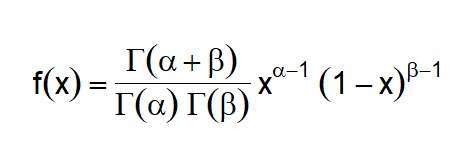
\includegraphics[width=175px]{C:/Users/marct/OneDrive - Tecnocampus Mataro-Maresme/Documentos/UNI_ESTADISTICA/2o/PRIMER CUATRIMESTRE/INFERENCIA ESTADISTICA I/TRABAJOS/INFERENCIA-I/TRABAJO EMPIRICO/LATEX Y FÓRMULAS/FUNCIÓN DE DENSIDAD/DENSIDAD1} \end{center}

También se puede escribir como:

\hypertarget{forma-de-la-distribuciuxf3n-beta}{%
\subsection{2.0 Forma de la distribución
Beta}\label{forma-de-la-distribuciuxf3n-beta}}

\begin{center}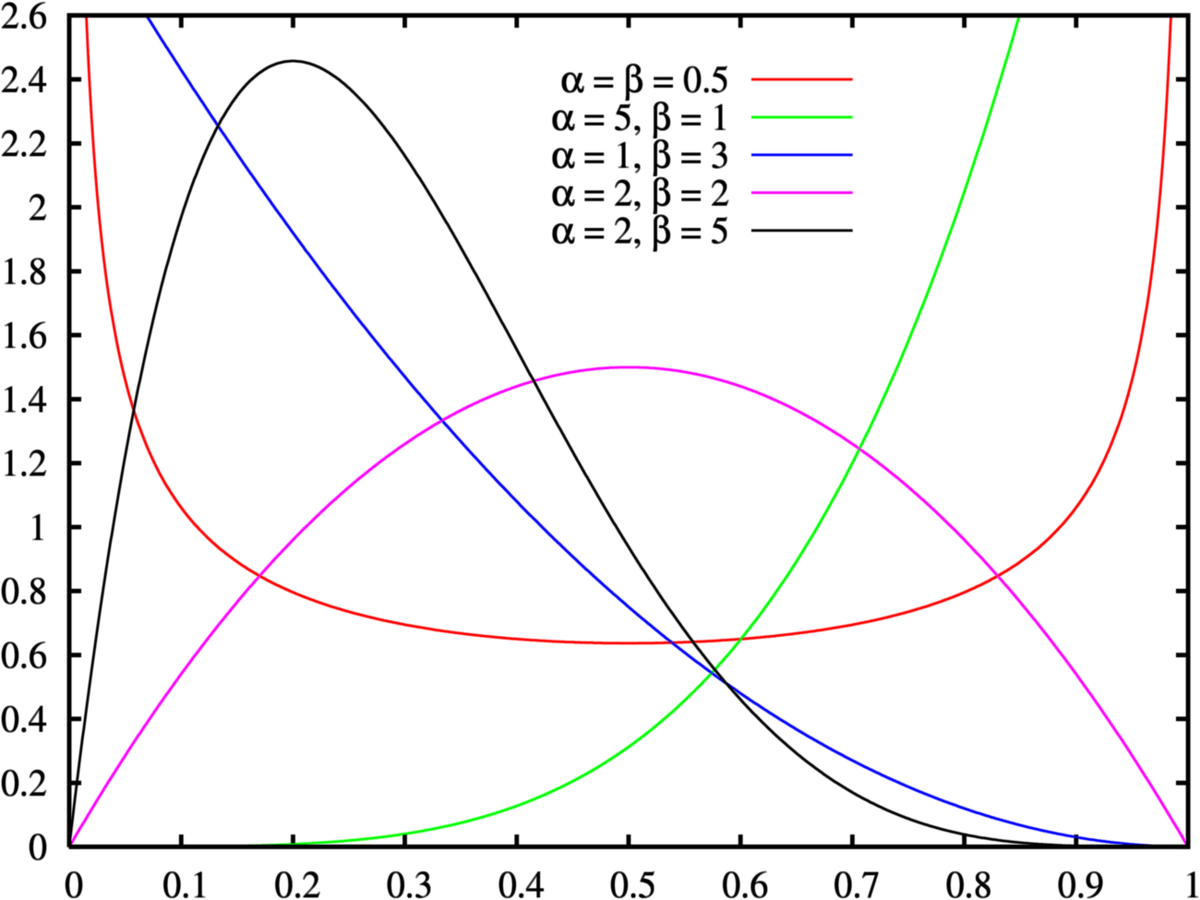
\includegraphics[width=175px]{C:/Users/marct/OneDrive - Tecnocampus Mataro-Maresme/Documentos/UNI_ESTADISTICA/2o/PRIMER CUATRIMESTRE/INFERENCIA ESTADISTICA I/TRABAJOS/INFERENCIA-I/TRABAJO EMPIRICO/IMAGENES/Beta_distribution} \end{center}

\hypertarget{momentos}{%
\subsection{2.1 Momentos}\label{momentos}}

\hypertarget{funciuxf3n-generadora-de-momentos}{%
\subsection{2.2 Función Generadora de
Momentos}\label{funciuxf3n-generadora-de-momentos}}

\hypertarget{creaciuxf3n-del-estaduxedstico-para-estimar-la-media-poblacional}{%
\section{3. Creación del Estadístico para estimar la Media
Poblacional}\label{creaciuxf3n-del-estaduxedstico-para-estimar-la-media-poblacional}}

En primer lugar hemos creado la función \emph{muestreo}. Esta función es
la base de toda la práctica, ya que nos permite crear muestras
aleatorias, calcular nuestro Estadístico, y la media muestral en cada
una de esas 40 muestras, etc.

\begin{Shaded}
\begin{Highlighting}[]
\KeywordTok{library}\NormalTok{(tidyverse)}
\KeywordTok{library}\NormalTok{(e1071)}
\KeywordTok{library}\NormalTok{(moments)}
\KeywordTok{library}\NormalTok{(gt)}
\KeywordTok{library}\NormalTok{(ggpubr)}
\KeywordTok{library}\NormalTok{(ggplotify)}
\KeywordTok{library}\NormalTok{(grid)}

\NormalTok{muestreo <-}\StringTok{ }\ControlFlowTok{function}\NormalTok{(alpha, beta)\{}
\NormalTok{        lista <-}\StringTok{ }\KeywordTok{list}\NormalTok{()}
\NormalTok{        tabla_muestras <-}\StringTok{ }\KeywordTok{matrix}\NormalTok{(}\DataTypeTok{ncol =} \DecValTok{40}\NormalTok{, }\DataTypeTok{nrow =} \DecValTok{10}\NormalTok{) }\OperatorTok\StringTok{ }\KeywordTok{as.data.frame}\NormalTok{() }
\NormalTok{        lista[[}\DecValTok{6}\NormalTok{]] <-}\StringTok{ }\KeywordTok{matrix}\NormalTok{(}\DataTypeTok{ncol =} \DecValTok{40}\NormalTok{, }\DataTypeTok{nrow =} \DecValTok{1}\NormalTok{) }\OperatorTok\StringTok{ }\KeywordTok{as.data.frame}\NormalTok{()}
\NormalTok{        media_poblacional <-}\StringTok{ }\NormalTok{alpha }\OperatorTok{/}\StringTok{ }\NormalTok{(alpha }\OperatorTok{+}\StringTok{ }\NormalTok{beta)}
\NormalTok{        varianza_poblacional <-}\StringTok{ }\NormalTok{alpha }\OperatorTok{*}\StringTok{ }\NormalTok{beta }\OperatorTok{/}\StringTok{ }\NormalTok{(((alpha }\OperatorTok{+}\StringTok{ }\NormalTok{beta) }\OperatorTok{^}\StringTok{ }\DecValTok{2}\NormalTok{ ) }\OperatorTok{*}\StringTok{ }\NormalTok{(alpha }\OperatorTok{+}\StringTok{ }\NormalTok{beta }\OperatorTok{+}\StringTok{ }\DecValTok{1}\NormalTok{))}
        \ControlFlowTok{for}\NormalTok{(j }\ControlFlowTok{in} \DecValTok{1}\OperatorTok{:}\DecValTok{40}\NormalTok{)\{}
                \KeywordTok{set.seed}\NormalTok{(j)}
\NormalTok{                tabla_muestras[, j] <-}\StringTok{ }\KeywordTok{rbeta}\NormalTok{(}\DecValTok{10}\NormalTok{, }\DataTypeTok{shape1 =}\NormalTok{ alpha, }\DataTypeTok{shape2 =}\NormalTok{ beta)}
                \KeywordTok{colnames}\NormalTok{(tabla_muestras)[j] <-}\StringTok{ }\KeywordTok{as.numeric}\NormalTok{(}\KeywordTok{gsub}\NormalTok{(}\StringTok{"V"}\NormalTok{, }\StringTok{""}\NormalTok{, }
                                                               \KeywordTok{colnames}\NormalTok{(tabla_muestras)[j]))}
                \KeywordTok{colnames}\NormalTok{(lista[[}\DecValTok{6}\NormalTok{]])[j] <-}\StringTok{  }\KeywordTok{as.numeric}\NormalTok{(}\KeywordTok{gsub}\NormalTok{(}\StringTok{"V"}\NormalTok{, }\StringTok{""}\NormalTok{, }
                                                            \KeywordTok{colnames}\NormalTok{(tabla_muestras)[j]))}
\NormalTok{                lista[[}\DecValTok{6}\NormalTok{]][, j] <-}\StringTok{ }\FloatTok{0.5}\OperatorTok{*}\NormalTok{(}\KeywordTok{quantile}\NormalTok{(tabla_muestras[, j], }
                                                 \DataTypeTok{probs =} \KeywordTok{c}\NormalTok{(}\FloatTok{0.6}\NormalTok{)) }\OperatorTok{+}\StringTok{ }
\StringTok{                                                }\KeywordTok{quantile}\NormalTok{(tabla_muestras[, j], }
                                                         \DataTypeTok{probs =} \KeywordTok{c}\NormalTok{(}\FloatTok{0.4}\NormalTok{)))}
\NormalTok{        \}}
\NormalTok{        lista[[}\DecValTok{1}\NormalTok{]] <-}\StringTok{ }\NormalTok{tabla_muestras}
\NormalTok{        lista[[}\DecValTok{2}\NormalTok{]] <-}\StringTok{ }\NormalTok{media_poblacional}
\NormalTok{        lista[[}\DecValTok{3}\NormalTok{]] <-}\StringTok{ }\NormalTok{varianza_poblacional}
\NormalTok{        lista[[}\DecValTok{4}\NormalTok{]] <-}\StringTok{ }\KeywordTok{data.frame}\NormalTok{(}\DataTypeTok{Muestra =} \KeywordTok{names}\NormalTok{(}\KeywordTok{colMeans}\NormalTok{(tabla_muestras)), }
                                 \DataTypeTok{mediamuestral =} \KeywordTok{unname}\NormalTok{(}\KeywordTok{colMeans}\NormalTok{(tabla_muestras))) }
\NormalTok{        lista[[}\DecValTok{5}\NormalTok{]] <-}\StringTok{ }\KeywordTok{data.frame}\NormalTok{(}\DataTypeTok{Estimador =} \StringTok{"Media Muestral"}\NormalTok{, }
                                 \DataTypeTok{Media =} \KeywordTok{mean}\NormalTok{(lista[[}\DecValTok{4}\NormalTok{]][, }\DecValTok{2}\NormalTok{]),}
                                 \DataTypeTok{Mediana =} \KeywordTok{median}\NormalTok{(lista[[}\DecValTok{4}\NormalTok{]][, }\DecValTok{2}\NormalTok{]),}
                                 \DataTypeTok{SD =} \KeywordTok{sd}\NormalTok{(lista[[}\DecValTok{4}\NormalTok{]][, }\DecValTok{2}\NormalTok{]), }
                                 \DataTypeTok{IQR =} \KeywordTok{IQR}\NormalTok{(lista[[}\DecValTok{4}\NormalTok{]][, }\DecValTok{2}\NormalTok{]), }
                                 \DataTypeTok{MAD =} \KeywordTok{mad}\NormalTok{(lista[[}\DecValTok{4}\NormalTok{]][, }\DecValTok{2}\NormalTok{]), }
                                 \DataTypeTok{Curtosis =}\NormalTok{ moments}\OperatorTok{::}\KeywordTok{kurtosis}\NormalTok{(lista[[}\DecValTok{4}\NormalTok{]][, }\DecValTok{2}\NormalTok{]), }
\NormalTok{                                 Asimetrí}\DataTypeTok{a =}\NormalTok{ e1071}\OperatorTok{::}\KeywordTok{skewness}\NormalTok{(lista[[}\DecValTok{4}\NormalTok{]][, }\DecValTok{2}\NormalTok{]))}
\NormalTok{        lista[[}\DecValTok{6}\NormalTok{]] <-}\StringTok{ }\KeywordTok{gather}\NormalTok{(}\KeywordTok{as.data.frame}\NormalTok{(lista[[}\DecValTok{6}\NormalTok{]])) }
        \KeywordTok{colnames}\NormalTok{(lista[[}\DecValTok{6}\NormalTok{]]) <-}\StringTok{ }\KeywordTok{c}\NormalTok{(}\StringTok{"Muestra"}\NormalTok{, }\StringTok{"Estadístico"}\NormalTok{)}
\NormalTok{        lista[[}\DecValTok{7}\NormalTok{]] <-}\StringTok{ }\KeywordTok{data.frame}\NormalTok{(}\DataTypeTok{Estimador =} \StringTok{"Estadístico"}\NormalTok{,}
                                 \DataTypeTok{Media =} \KeywordTok{mean}\NormalTok{(lista[[}\DecValTok{6}\NormalTok{]][, }\DecValTok{2}\NormalTok{]),}
                                 \DataTypeTok{Mediana =} \KeywordTok{median}\NormalTok{(lista[[}\DecValTok{6}\NormalTok{]][, }\DecValTok{2}\NormalTok{]),}
                                 \DataTypeTok{SD =} \KeywordTok{sd}\NormalTok{(lista[[}\DecValTok{6}\NormalTok{]][, }\DecValTok{2}\NormalTok{]), }
                                 \DataTypeTok{IQR =} \KeywordTok{IQR}\NormalTok{(lista[[}\DecValTok{6}\NormalTok{]][, }\DecValTok{2}\NormalTok{]), }
                                 \DataTypeTok{MAD =} \KeywordTok{mad}\NormalTok{(lista[[}\DecValTok{6}\NormalTok{]][, }\DecValTok{2}\NormalTok{]), }
                                 \DataTypeTok{Curtosis =}\NormalTok{ moments}\OperatorTok{::}\KeywordTok{kurtosis}\NormalTok{(lista[[}\DecValTok{6}\NormalTok{]][, }\DecValTok{2}\NormalTok{]), }
\NormalTok{                                 Asimetrí}\DataTypeTok{a =}\NormalTok{ e1071}\OperatorTok{::}\KeywordTok{skewness}\NormalTok{(lista[[}\DecValTok{6}\NormalTok{]][, }\DecValTok{2}\NormalTok{]))}
\NormalTok{        lista[[}\DecValTok{8}\NormalTok{]] <-}\StringTok{ }\KeywordTok{rbind}\NormalTok{(lista[[}\DecValTok{5}\NormalTok{]], lista[[}\DecValTok{7}\NormalTok{]])}
        \KeywordTok{names}\NormalTok{(lista) <-}\StringTok{ }\KeywordTok{c}\NormalTok{(}\StringTok{"tabla_muestras"}\NormalTok{, }\StringTok{"media_poblacional"}\NormalTok{, }
                          \StringTok{"varianza_poblacional"}\NormalTok{, }\StringTok{"media_muestral"}\NormalTok{, }
                          \StringTok{"medidas_media_muestral"}\NormalTok{, }\StringTok{"estadistico"}\NormalTok{, }
                          \StringTok{"medidas_estadistico"}\NormalTok{, }\StringTok{"tabla_comparacion"}\NormalTok{)}
\NormalTok{        lista}
\NormalTok{\}}

\NormalTok{resultados <-}\StringTok{ }\KeywordTok{muestreo}\NormalTok{(}\DataTypeTok{alpha =} \DecValTok{2}\NormalTok{, }\DataTypeTok{beta =} \DecValTok{2}\NormalTok{)}

\NormalTok{datosgrafico <-}\StringTok{ }\KeywordTok{inner_join}\NormalTok{(resultados}\OperatorTok{$}\NormalTok{media_muestral , resultados}\OperatorTok{$}\NormalTok{estadistico)}
\end{Highlighting}
\end{Shaded}

\hypertarget{evaluaciuxf3n-de-nuestro-estaduxedstico}{%
\section{4. Evaluación de nuestro
Estadístico}\label{evaluaciuxf3n-de-nuestro-estaduxedstico}}

\hypertarget{tabla-de-medidas-falta-pasar-a-formato-leible-por-un-pdf-es-decir-eliminar-lo-de-gt}{%
\subsection{4.1 Tabla de Medidas (falta pasar a formato leible por un
pdf, es decir eliminar lo de
gt)}\label{tabla-de-medidas-falta-pasar-a-formato-leible-por-un-pdf-es-decir-eliminar-lo-de-gt}}

\newpage

\hypertarget{histogramas}{%
\subsection{4.2 Histogramas}\label{histogramas}}

\begin{Shaded}
\begin{Highlighting}[]
\NormalTok{grafico_estadistico_histogram <-}\StringTok{ }\KeywordTok{ggplot}\NormalTok{(}\DataTypeTok{data =}\NormalTok{ datosgrafico, }
                                        \KeywordTok{aes}\NormalTok{(}\DataTypeTok{x =}\NormalTok{ Estadístico)) }\OperatorTok{+}\StringTok{ }
\StringTok{        }\KeywordTok{geom_histogram}\NormalTok{(}\DataTypeTok{fill =} \StringTok{"lightblue"}\NormalTok{, }\DataTypeTok{binwidth =} \FloatTok{0.05}\NormalTok{, }\DataTypeTok{color =} \StringTok{"black"}\NormalTok{) }\OperatorTok{+}\StringTok{ }
\StringTok{        }\KeywordTok{ggtitle}\NormalTok{(}\StringTok{"Histograma de nuestro Estadístico"}\NormalTok{) }\OperatorTok{+}\StringTok{ }
\StringTok{        }\KeywordTok{geom_vline}\NormalTok{(}\KeywordTok{aes}\NormalTok{(}\DataTypeTok{xintercept =}\NormalTok{ resultados[[}\DecValTok{7}\NormalTok{]]}\OperatorTok{$}\NormalTok{Media, }\DataTypeTok{col =} \StringTok{"Estimador"}\NormalTok{), }
                   \DataTypeTok{linetype =} \StringTok{"dashed"}\NormalTok{, }\DataTypeTok{size =} \DecValTok{1}\NormalTok{) }\OperatorTok{+}
\StringTok{        }\KeywordTok{geom_vline}\NormalTok{(}\KeywordTok{aes}\NormalTok{(}\DataTypeTok{xintercept =}\NormalTok{ resultados}\OperatorTok{$}\NormalTok{media_poblacional,  }
                       \DataTypeTok{col =} \StringTok{"Media Poblacional"}\NormalTok{), }\DataTypeTok{size =} \DecValTok{1}\NormalTok{) }\OperatorTok{+}\StringTok{ }
\StringTok{        }\KeywordTok{scale_color_manual}\NormalTok{(}\DataTypeTok{name =} \StringTok{""}\NormalTok{, }
                           \DataTypeTok{values =} \KeywordTok{c}\NormalTok{(}\StringTok{"Media Poblacional"}\NormalTok{ =}\StringTok{ "black"}\NormalTok{, }
                                      \DataTypeTok{Estimador =} \StringTok{"red"}\NormalTok{)) }\OperatorTok{+}\StringTok{ }
\StringTok{        }\KeywordTok{xlab}\NormalTok{(}\StringTok{"x"}\NormalTok{) }\OperatorTok{+}\StringTok{ }\KeywordTok{ylab}\NormalTok{(}\StringTok{"f(x)"}\NormalTok{) }\OperatorTok{+}
\StringTok{        }\KeywordTok{theme}\NormalTok{(}\DataTypeTok{legend.position =} \StringTok{"top"}\NormalTok{,}
              \DataTypeTok{legend.text =} \KeywordTok{element_text}\NormalTok{(}\DataTypeTok{size =} \DecValTok{14}\NormalTok{),}
              \DataTypeTok{axis.text.x =} \KeywordTok{element_text}\NormalTok{(}\DataTypeTok{size =} \DecValTok{12}\NormalTok{),}
              \DataTypeTok{axis.text.y =} \KeywordTok{element_text}\NormalTok{(}\DataTypeTok{size =} \DecValTok{12}\NormalTok{),}
              \DataTypeTok{axis.title =} \KeywordTok{element_text}\NormalTok{(}\DataTypeTok{size =} \DecValTok{13}\NormalTok{, }\DataTypeTok{face =} \StringTok{"bold"}\NormalTok{), }
              \DataTypeTok{plot.title =} \KeywordTok{element_text}\NormalTok{(}\DataTypeTok{size =} \DecValTok{18}\NormalTok{, }\DataTypeTok{face =} \StringTok{'bold'}\NormalTok{, }
                                        \DataTypeTok{hjust =} \FloatTok{0.5}\NormalTok{)) }\OperatorTok{+}\StringTok{ }
\StringTok{        }\KeywordTok{xlim}\NormalTok{(}\DecValTok{0}\NormalTok{, }\DecValTok{1}\NormalTok{)}
\NormalTok{grafico_estadistico_histogram}
\end{Highlighting}
\end{Shaded}

\begin{center}\includegraphics{TRABAJO-BETA_files/figure-latex/unnamed-chunk-6-1} \end{center}

\end{document}
